\subsection{Sviluppo}

\subsubsection{Descrizione e Scopo}
Il processo di sviluppo rappresenta l’insieme delle attività necessarie per realizzare il prodotto software, garantendo il rispetto dei requisiti e delle scadenze concordate con il proponente. Questo processo si articola in diverse fasi fondamentali, quali l'analisi dei requisiti, la progettazione, la codifica, l'integrazione, e la verifica, assicurando che ogni fase contribuisca al raggiungimento degli obiettivi prefissati.
Le linee guida descritte in questa sezione sono volte a strutturare il lavoro in modo chiaro e uniforme, promuovendo la qualità del prodotto finale. Seguendo standard solidi e definiti, nel caso specifico l'ISO/IEC 12207:1995, si crea un ambiente di lavoro orientato a garantire la coerenza nei metodi utilizzati e il rispetto delle aspettative.
L'obiettivo è consegnare un prodotto software di alta qualità, che soddisfi le esigenze richieste, rispettando le tempistiche e garantendo il successo del progetto.\\

\subsubsection{Analisi dei Requisiti}
L’analisi dei requisiti è la prima fase cruciale del processo di sviluppo software. Lo scopo principale di questa fase è definire con chiarezza le funzionalità e le caratteristiche che il sistema dovrà offrire, in base alle necessità degli utenti. Per raggiungere tale obiettivo, è essenziale stabilire una comunicazione efficace con il proponente, assicurandosi che tutte le esigenze siano documentate e validate. Questo processo permette di chiarire gli obiettivi del prodotto, identificare i vincoli operativi e fornire ai Progettisti le informazioni necessarie per sviluppare un’architettura coerente e un design adeguato.
Il risultato di questa attività è formalizzato nel documento \textit{Analisi\_dei\_requisiti.pdf}, redatto dagli Analisti, che contiene una descrizione dettagliata degli obiettivi del prodotto, delle funzionalità previste, delle caratteristiche degli utenti e delle tecnologie coinvolte. Include inoltre una sezione dedicata ai casi d’uso, che descrivono le interazioni tra gli attori esterni e il sistema.
Infine, l’analisi dei requisiti contribuisce a migliorare la comunicazione tra tutti gli stakeholder, agevola la pianificazione del progetto in termini di tempistiche e costi e fornisce un riferimento chiaro per le attività di verifica e test.\\

\paragraph{Casi d'uso}
I casi d’uso rappresentano scenari concreti che descrivono come gli utenti e altri attori interagiranno con il sistema per raggiungere obiettivi specifici. Questi scenari aiutano a identificare requisiti chiave e prevenire malintesi. È importante sottolineare che i diagrammi dei casi d’uso non si concentrano sui dettagli implementativi. Il loro scopo è quello di rappresentare la funzionalità del sistema esclusivamente dal punto di vista esterno, evidenziando come esso interagisce con gli attori e soddisfa le loro esigenze.\\

\medskip Ogni caso d'uso ha le seguenti caratteristiche:

\begin{enumerate}
    \item \textbf{Identificativo:} UC [Numero caso d’uso] . [Numero sottocaso d’uso] - [Titolo]\\
    \medskip Dove:
    \begin{itemize}
        \item \textbf{Numero caso d’uso:} ID relativo al caso d'uso pricnipale.
        \item \textbf{Numero sottocaso d’uso:} ID relativo allo specifico sottocaso d'uso (se applicabile).
        \item \textbf{Titolo:} descrizione breve ed esplicativa.
    \end{itemize}

    \item \textbf{Attore principale:} L'entità che interagisce attivamente con il sistema, ad esempio un utente specifico o un altro sistema esterno.

    \item \textbf{Attore secondario:} Eventuale entità esterna che non interagisce attivamente con il sistema, ma permette al sistema di soddisfare il bisogno dell’attore principale.

    \item \textbf{Descrizione:} Breve descrizione della funzionalità del caso d’uso.

    \item \textbf{Scenario principale:} Sequenza di eventi che si susseguono da quando un attore inizia ad interagire con il sistema.

    \item \textbf{Precondizioni:} Descrizione dello stato necessario per attivare il caso d’uso.

    \item \textbf{Postcondizioni:} Descrizione dello stato del sistema al termine del caso d’uso.

    \item \textbf{Estensioni:} Eventuali scenari alternativi, descritti in questa sezione se presenti.

    \item \textbf{User story associata:} Funzionalità software descritta dal punto di vista dell'utente, definita nella forma:
    \begin{quote}
        Come [utente], desidero poter [funzionalità] per [valore aggiunto].
    \end{quote}
\end{enumerate}

\paragraph{Diagrammi dei casi d'uso} I diagrammi dei casi d'uso sono strumenti visivi che rappresentano le funzionalità del sistema dal punto di vista dell'utente. Mostrano come gli attori esterni (utenti, dispositivi, altri sistemi) interagiscono con il sistema, senza entrare nei dettagli tecnici. Il loro obiettivo principale è descrivere le interazioni tra attori e sistema, facilitando la comprensione dei requisiti funzionali e la comunicazione tra gli stakeholder. Ogni caso d'uso descrive una sequenza di azioni che un attore compie per raggiungere un obiettivo specifico. Questi casi sono interconnessi e rappresentano i flussi di lavoro principali, evidenziando come l'utente interagisce con il sistema. I diagrammi non trattano i dettagli implementativi, ma si concentrano sulle funzionalità, trattando il sistema come un "black box" esterno.\\
\medskip Di seguito sono elencati i principali componenti di un diagramma dei casi d’uso:

\begin{itemize}
    \item \textbf{Attori}\\
        Gli attori sono entità esterne al sistema che interagiscono con esso per utilizzare le sue funzionalità. Possono essere utenti umani, altri sistemi software, dispositivi, macchine o organizzazioni. Un caso d'uso definisce una specifica funzionalità che il sistema fornisce agli attori, senza entrare nei dettagli implementativi. Nel diagramma dei casi d'uso, gli attori sono rappresentati da figure stilizzate posizionate all'esterno del rettangolo che delinea il sistema, e ciascuno è identificato da un’etichetta con il suo nome.
        \begin{figure}[H]
        \centering
        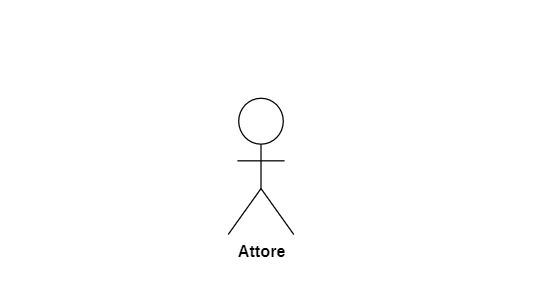
\includegraphics[width=0.45\textwidth]{Attore.PNG}
        \caption{Rappresentazione di un attore.}
        \end{figure}

        \item \textbf{Casi d'uso}\\
        Ogni caso d’uso identifica una specifica azione o funzionalità offerta dal sistema, con cui l’attore può interagire. I casi d'uso sono collegati tramite una linea continua agli attori che hanno accesso a quella funzionalità, creando una chiara relazione tra gli utenti e le azioni che possono compiere. Nel diagramma dei casi d’uso, ogni caso è rappresentato da una forma ovale contenente un ID univoco e un titolo esplicativo.
        \begin{figure}[H]
        \centering
        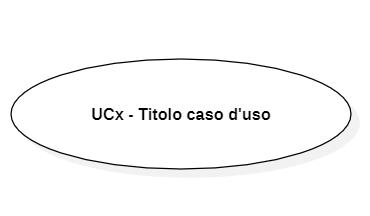
\includegraphics[width=0.35\textwidth]{UC.PNG}
        \caption{Rappresentazione di un caso d'uso.}
        \end{figure}

        \item \textbf{Sottocasi d'uso}\\
        Un sottocaso d’uso rappresenta una versione più dettagliata di un caso d’uso  generico. Esso offre un livello di dettaglio più approfondito sulle funzionalità o sui particolari scenari di utilizzo rispetto al caso d’uso principale. Non è obbligatorio per un caso d'uso possedere uno o più sottocasi.
        \begin{figure}[H]
        \centering
        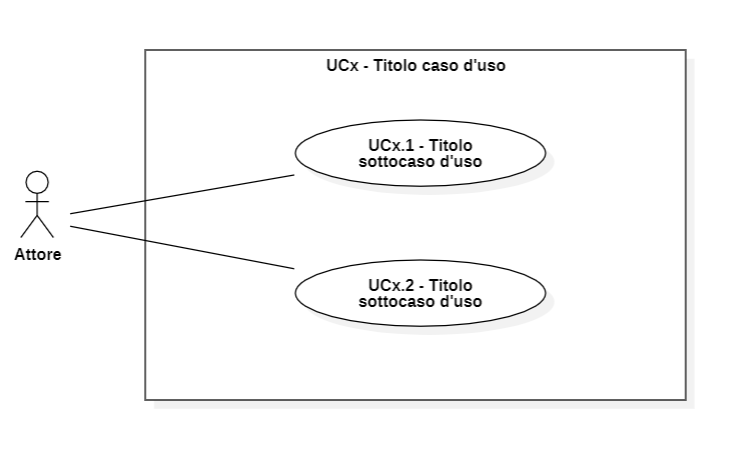
\includegraphics[width=0.6\textwidth]{SottocasoD'Uso.PNG}
        \caption{Rappresentazione di un sottocaso d'uso.}
        \end{figure}

        \item \textbf{Sistema}\\
         Il sistema viene rappresentato con un rettangolo all'interno del quale vengono collocati i casi d'uso. All'esterno del rettangolo sono invece posizionati i vari attori.
        \begin{figure}[H]
        \centering
        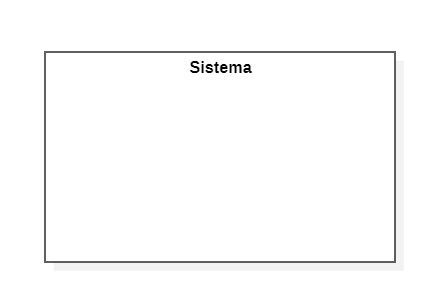
\includegraphics[width=0.5\textwidth]{Sistema.PNG}
        \caption{Rappresentazione di un sistema.}
        \end{figure}

        \item \textbf{Associazione}\\
        Una linea di associazione stabilisce una connessione tra un attore e un caso d'uso quando l'attore è coinvolto nell'attività descritta dal caso d'uso. Questo collegamento visivo rappresenta il ruolo dell'attore nell'attivare o nell'utilizzare una specifica funzionalità del sistema.
        \begin{figure}[H]
        \centering
        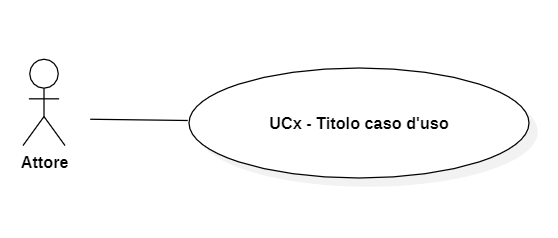
\includegraphics[width=0.5\textwidth]{Associazione.PNG}
        \caption{Rappresentazione di un sistema.}
        \end{figure}

        \item \textbf{Generalizzazione (attori)}\\
        La generalizzazione tra attori rappresenta una relazione gerarchica in cui un attore specializzato (figlio) eredita comportamenti e caratteristiche da un attore base (genitore). Questo meccanismo aiuta a organizzare gerarchicamente gli attori nei diagrammi dei casi d’uso, definendo i casi d'uso che un attore può utilizzare e che sono anche disponibili per gli attori più specializzati. La generalizzazione viene rappresentata con una linea solida e una freccia vuota che va dall'attore figlio all'attore genitore, indicando la direzione dell'eredità.
        \begin{figure}[H]
        \centering
        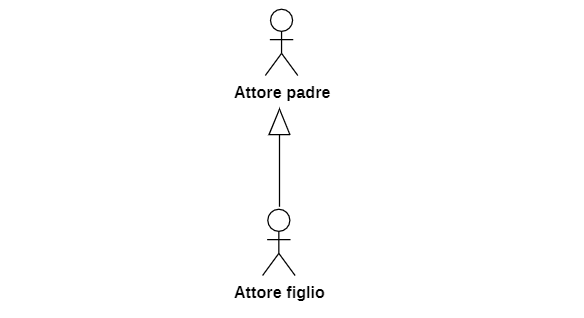
\includegraphics[width=0.6\textwidth]{GeneralizzazioneAttori.PNG}
        \caption{Rappresentazione di un sistema.}
        \end{figure}

        \item \textbf{Inclusione}\\
        La relazione di inclusione indica quando un caso d'uso (includente) comprende l'esecuzione di un altro caso d'uso (incluso). Quando un attore interagisce con il caso d'uso includente, il caso d'uso incluso viene eseguito automaticamente come parte di quest'ultimo. Questa relazione è utile per il riutilizzo delle funzionalità e per evitare la duplicazione delle stesse logiche in più casi d'uso. La relazione di inclusione viene rappresentata da una freccia tratteggiata che collega il caso d'uso incluso al caso d'uso includente.
        \begin{figure}[H]
        \centering
        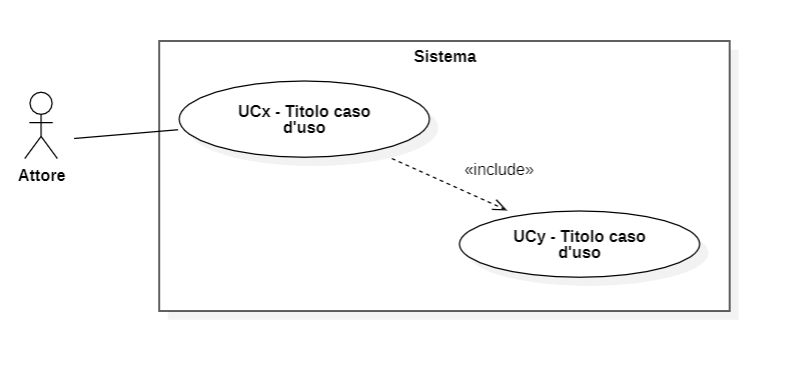
\includegraphics[width=0.6\textwidth]{Inclusione.PNG}
        \caption{Rappresentazione di un sistema.}
        \end{figure}

        \item \textbf{Estensione}\\
        La relazione di estensione indica quando un caso d'uso (estendente) può modificare o arricchire il comportamento di un altro caso d'uso (esteso) in determinate circostanze. Questa relazione viene utilizzata quando un evento o una condizione porta il flusso del caso d'uso a deviare dallo scenario principale verso uno scenario alternativo, come nei casi di errore, ma mantenendo le stesse precondizioni del caso d'uso principale. La relazione di estensione è rappresentata da una freccia tratteggiata che collega il caso d'uso estendente al caso d'uso esteso.
        \begin{figure}[H]
        \centering
        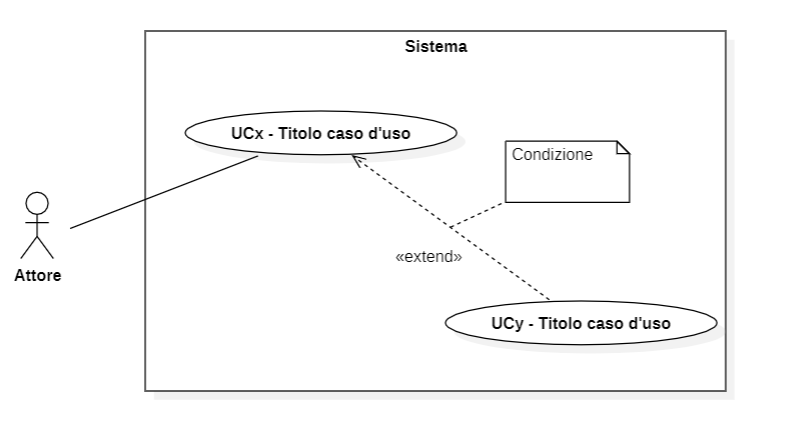
\includegraphics[width=0.6\textwidth]{Estensione.PNG}
        \caption{Rappresentazione di un sistema.}
        \end{figure}

        \item \textbf{Generalizzazione (casi d'uso)}\\
        La generalizzazione nei diagrammi dei casi d’uso rappresenta una relazione di ereditarietà tra casi d’uso, in cui un caso d’uso più specifico eredita il comportamento da un caso d’uso più generico. Questa relazione è utile per definire funzionalità più dettagliate, ed è simboleggiata da una linea con una freccia vuota che va dal caso d'uso specifico al caso d'uso generico.
        \begin{figure}[H]
        \centering
        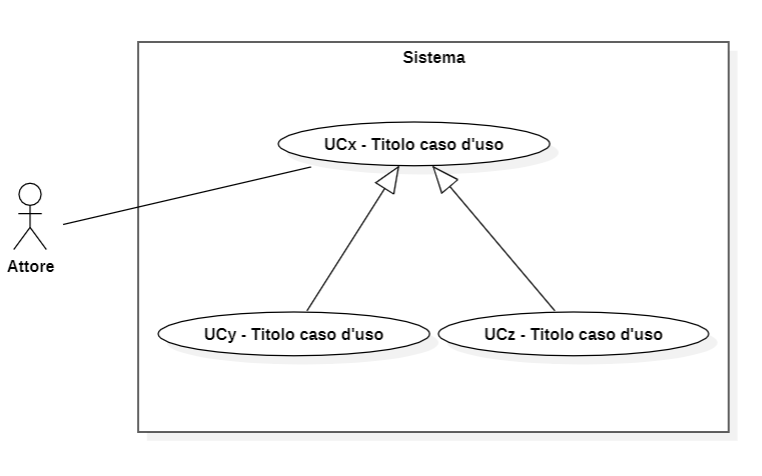
\includegraphics[width=0.6\textwidth]{GeneralizzazioneUC.PNG}
        \caption{Rappresentazione di un sistema.}
        \end{figure}
\end{itemize}

\paragraph{Requisiti}

\paragraph{Metriche}

\subsubsection{Progettazione}

\subsubsection{Codifica}

\subsubsection{Integrazione}

\subsubsection{Verifica}


